%Discussion
\chapter{Results}

In this chapter, we evaluate the performance of the proposed adaptive cruise system via computer simulations.

\section{Simulation Setup}

In simulations, we used the commercial software PreScan which models vehicle dynamics in real time [15]. We generated the environment in order to train the DQN by simulating the random behavior of the pedestrian. In the simulations, we assume that the relative location of the pedestrian is provided to the agent. To make the system practical, we add slight measurement noise to it. In each episode, the initial position of vehicle is set to (0, 0). Time-to-collision T T C is chosen according to the uniform distrubution between 1.5 s and 4 s. The initial velocity of the vehicle is uniformly distributed between $v_{initmin} = 2.78 m/s (10 km/s)$ and $v_{initmax} = 16.67 m/s (60 km/h)$. At the beginning of the episodes, the position of the pedestrian is fixed to 5 ? $v_{init}$ meters away from the position of the vehicle. The pedestrian stands either at the far-side or at near-side of the vehicle with equal probability. The behavior of the pedestrian follows one of two scenarios below;

\begin{itemize}
\item Scenario 1 : Cross the road
\item Scenario 2 : Stay at initial position.
During training, either of two scenarios is selected with equal probability. In Scenario 1, the pedestrian starts to move when the vehicle is crossing at the ?pedestrian crossing point? ptrig = (5?TTC)?vinit. (see Fig. 4.) The safety distance l for the pedestrian is set to 3 m. The agent chooses the brake control among ahigh = ?9.8 m/s2, amid = ?5.9 m/s2, ahigh = ?2.9 m/s2 and anothing = 0 m/s2 every ?T = 0.1 second. The detailed simulation setup is summarized below.
\item Initial velocity of vehicle vinit ? U (2.78, 16.67) m/s ? Velocity of pedestrian vped ? U (2, 4) m/s
\item Time-to-collision T T C ? U (1.5, 4) s
\item Initial pedestrian position pedposx = 5 ? vinit m
\item Trigger point $p_{trig} = (5 TTC) ? v_{init} m$
\item Safety dist = 3 m
\item T=0.1s
\item $a_{high}, a_{mid}, a_{low}, a_{zero} = {9.8, 5.9, 2.9, 0} m/s^2$
\end{itemize}

\section{Training of DQN}

The neural network used for the DQN consists of the fully- connected layers with five hidden layers. RMSProp algorithm [14] is used to minimize the loss with learning rate ? = 0.0005. The number of position data samples used as a state is set to n = 5. We set the size of the replay memory to 10,000 and that of the trauma memory to 1,000. We set the replay batch size to 32 and trauma batch size to 10. The summary of the DQN configurations used for our experiments is provided below:

\begin{itemize}
\item State buffer size: n = 5
\item Network architecture: fully-connected feed-forward network
\item Nonlinear function: leaky ReLU [13]
\item Number of nodes for each layers : [17 (Input layer), 100, 70, 50, 70, 100, 27 (Output layer)]
\item RMSProp optimizer with learning rate 0.0005 [14]
\item Replay memory size: 10,000
\item Replay batch size: 32
\item Trauma memory size: 1,000
\item Trauma batch size = 10
\item Reward function: ? = 0.001, ? = 0.1, ? = 0.01, ? =100
\end{itemize}

Fig. 5 provides the plot of the total accumulated rewards i.e., value function achieved for each episode when training is conducted with and without trauma memory. We observe that with trauma memory the value function converges after 2,000 episodes and high total reward is steadily attained after convergence while without trauma memory the policy does not converge and keeps fluctuating.

\section{Visualizing the Value Function}

\begin{figure}[h]
\centering
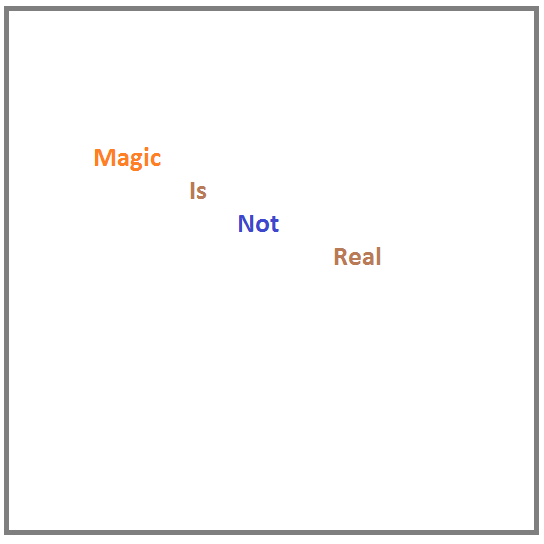
\includegraphics[width=0.5\textwidth]{figs/magic}
\caption{Achieved value function achieved during training.}
\end{figure}

Safety test was conducted for several different T T C values. Collision rate is measured for 10,000 trials for each TTC value. Table I provides the collision rate for each TTC value for the test performed for Scenario 1. The agent avoids collision successfully for TTC values above 1.5s. For the cases with TTC values less than 1.5s, we observe some collisions. According to our analysis on the trajectory of braking actions, these are the cases where collision was not avoidable due to the high initial velocity of the vehicle even though full braking actions were applied. The agent passed the pedestrian without unnecessary stop for all cases in the Scenario 2. The detailed trajectory of the brake actions for one example case is shown in Fig. 6. Fig. 6 (a) shows the trajectory of the position of the vehicle and the pedestrian recorded every 0.1 s. The velocity of the agent and the brake actions applied are shown in Fig. 6 (b) and (c), respectively. The vehicle starts to decelerate about 20 m away from the pedestrian and completely stops about 5 m ahead, thereby accomplishing collision avoidance. We observe that weak braking actions are applied in the beginning part of deceleration and then strong braking actions come as the agent gets close to the pedestrian.

Fig. 7 shows how the initial position of the pedestrian and the relative distance between the pedestrian and vehicle are distributed for 1,000 trials in the scenario 1. We see that the vehicle stops around 5 m in front of the pedestrian for most of cases. This seems to be reasonable safe braking operation considering the safety distance of l = 3 m. Note that this distance can be adjusted by changing the reward parameters. Overall, the experimental results show that the proposed autonomous braking system exhibits consistent brake control performance for all cases considered.

\section{Main Evaluation}

We compare our results with the best performing methods from the RL literature [3, 4]. The method labeled Sarsa used the Sarsa algorithm to learn linear policies on several different feature sets hand- engineered for the Atari task and we report the score for the best performing feature set [3]. Contingency used the same basic approach as Sarsa but augmented the feature sets with a learned representation of the parts of the screen that are under the agent?s control [4]. Note that both of these methods incorporate significant prior knowledge about the visual problem by using background sub- traction and treating each of the 128 colors as a separate channel. Since many of the Atari games use one distinct color for each type of object, treating each color as a separate channel can be similar to producing a separate binary map encoding the presence of each object type. In contrast, our agents only receive the raw RGB screenshots as input and must learn to detect objects on their own.


%\vfill
